\section{速度制御のための入力変換}

前章では4輪メカナムホイールロボットの逆運動学及び順運動学を導いた.
ロボットを操縦する際は,速度ベクトル$\vec{x} = (\dot{x}, \dot{y}, \dot{\theta})^T$を入力として,逆運動学により各ホイールの速度を計算するのが一般的だが,入力できる速度には制限がある.
メカナムホイールのような全方位移動ロボットのコントローラとしては3軸のジョイスティックが用いられるのが一般的であるが,それぞれのジョイスティックをそのまま各速度に対応させるのは適切ではない.
そこで,コントローラからの3軸入力を,ロボットへの入力速度ベクトルへとマッピングする処理が必要となる.

\subsection{入力速度の制約式}

ロボットの移動速度はホイールの最大回転速度により制限される.式\ref{eq:inv3}を見ると分かるように,ロボットへの入力速度$\dot{x}$,$\dot{y}$,$\dot{\theta}$は,その絶対値の和がホイールの出せる最大回転速度を超えるような組み合わせになってはならない.
ここで,各ホイールの性能は全て同等とし,ホイールが出せる最大角速度を$\omega_{\text{max}}$,ホイールの最大周速度を$V_{\text{max}} = r \omega_{\text{max}}$とすると,式\ref{eq:constraint}に示す入力速度の制約式が得られる.

\begin{equation}
  V_{\text{max}} = |\dot{x}| + |\dot{y}| + 2l|\dot{\theta}|
  \label{eq:constraint}
\end{equation}

ここで,$\hat{\dot{\theta}} = 2l\dot{\theta}$として式\ref{eq:constraint}に代入すると,式\ref{eq:constraint}は図に示すような$\dot{x}\dot{y}\hat{\dot{\theta}}$座標系における正八面体の内部領域を表す.
ロボットへの入力速度ベクトル$\vec{x} = (\dot{x}, \dot{y}, \dot{\theta})^T$をこの座標系の位置ベクトルであるとしたとき,位置ベクトルは正八面体の内部に存在していなければならない.

\begin{figure}[h]
  \centering
  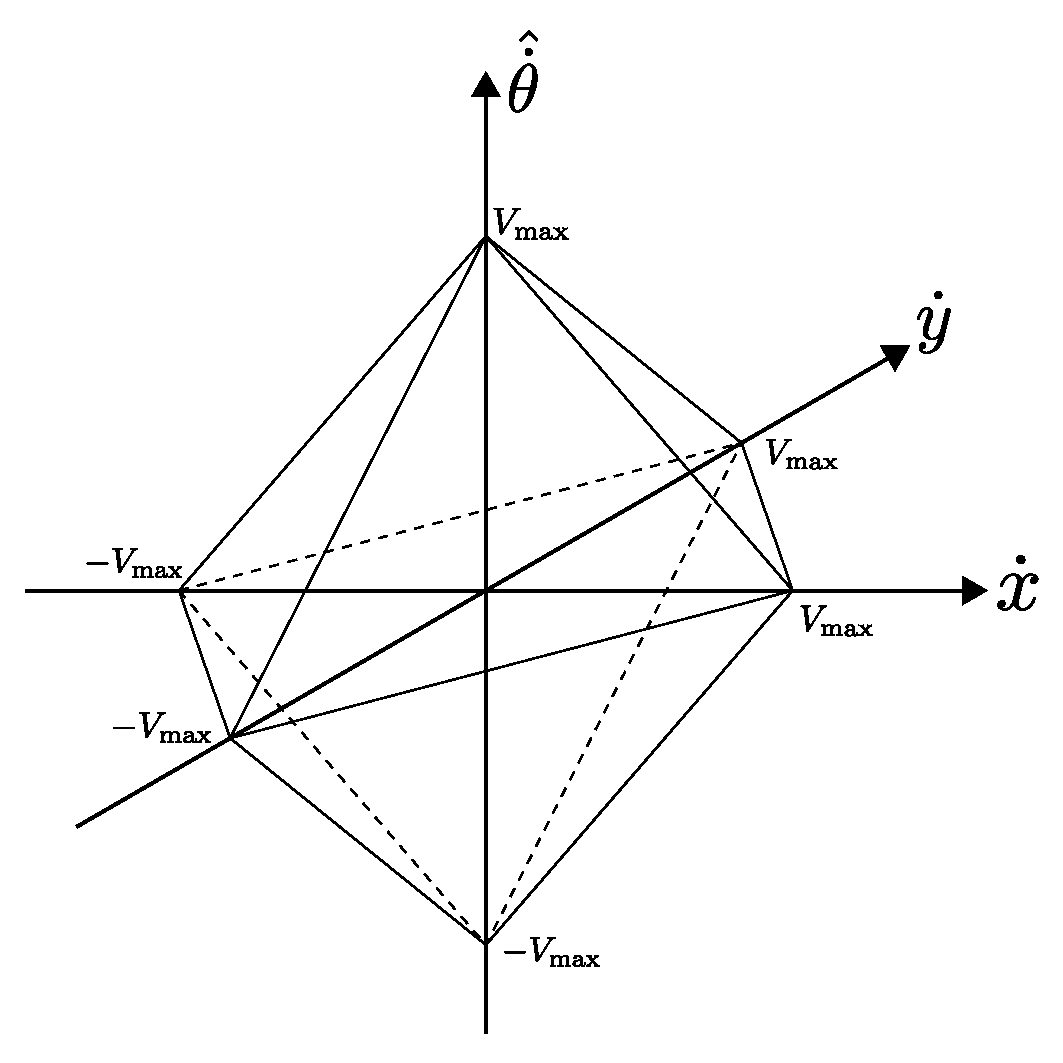
\includegraphics[width=80truemm, clip]{images/constraint.pdf}
  \caption{Constraint Area of Input Velocity Vector}
  \label{fig:constraint}
\end{figure}

\subsection{入力信号から速度ベクトルへのマッピング}

\subsubsection{コントローラからの入力信号}

ここでは3軸のアナログジョイスティックを用いてロボットを速度制御することを考える.
それぞれのアナログジョイスティックの入力は$\dot{x}$,$\dot{y}$,$\hat{\dot{\theta}}$に対応するものとし,$\dot{x}$に対応するアナログジョイスティックの信号値を$\alpha$,$\dot{y}$に対応するものを$\beta$,$\hat{\dot{\theta}}$に対応するものを$\gamma$と表す.
また,各ジョイスティックの信号値の範囲は-1.0~1.0であるとする.

3つのジョイスティックによる入力の組み合わせをベクトル$\vec{\epsilon} = (\alpha, \beta, \gamma)^T$で表す.
$\alpha\beta\gamma$座標系において,$\vec{\epsilon}$が取る領域は,原点を中心とする幅2の正方形となる.
この正方形の領域を,図\ref{fig:constraint}に示す正八面体にマッピングすることで,ジョイスティックによる制御が可能になる.

\begin{figure}[h]
  \centering
  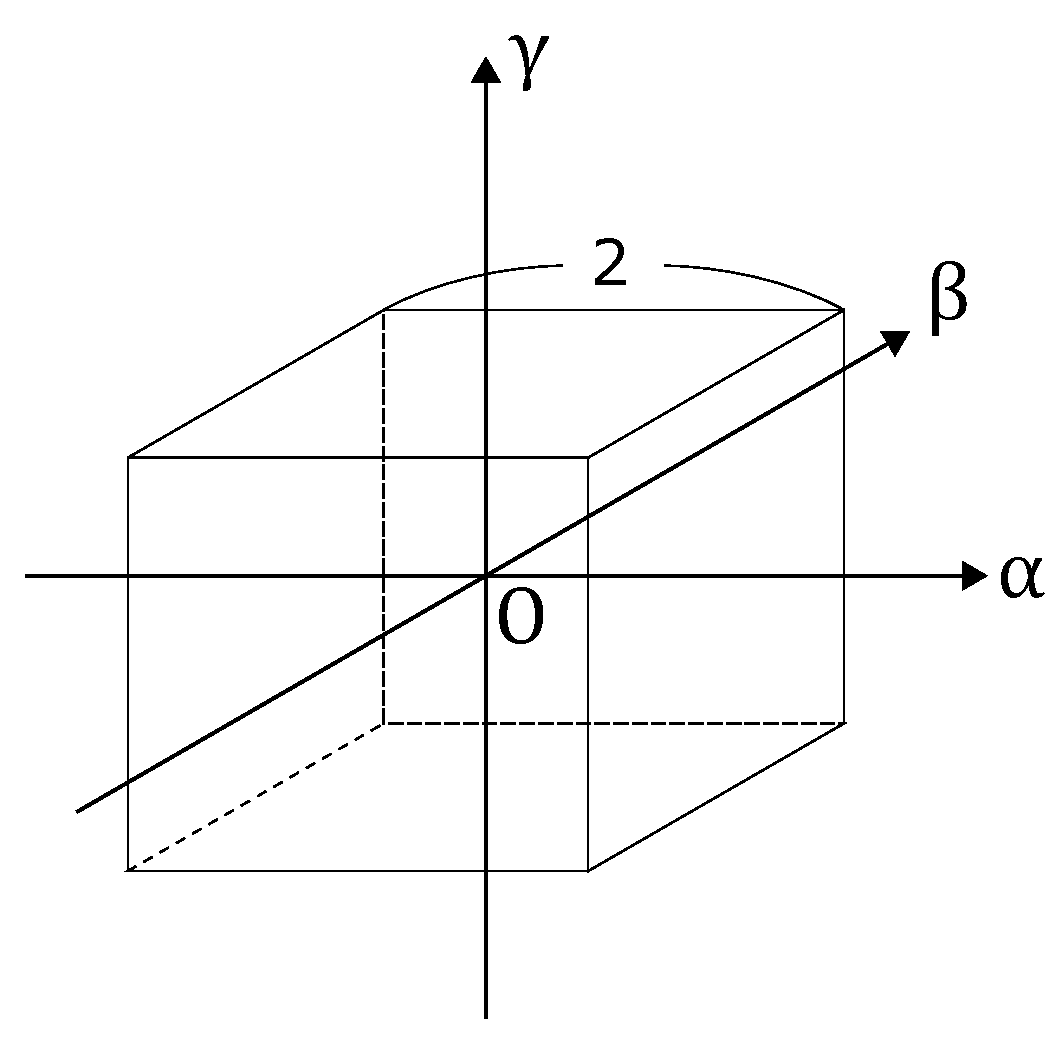
\includegraphics[width=80truemm, clip]{images/input.pdf}
  \caption{Input Area}
  \label{fig:input}
\end{figure}

\subsubsection{極座標変換によるアプローチ}

正方形領域から正八面体領域へのマッピングを直接行うのは困難であるため,ここでは極座標変換を用いたマッピング処理を行う.

まず,$\alpha\beta\gamma$座標系における正方形領域を3次元極座標における球面へ変換する.
入力信号ベクトル$\vec{\epsilon}$の向きと大きさを求める.